
% DICTIONARY;finite type ...;... skończonego typu;niezmiennik
Niezmienniki Wasiljewa (znane także jako niezmienniki skończonego typu) umożliwiają radykalnie nowe podejście do węzłów.
Około 1989 roku odkryli je niezależnie Wiktor Wasiljew, w~oparciu o~teorię osobliwości, oraz Michaił Gusarow, metodami kombinatorycznymi.
\index[persons]{Wasiljew, Wiktor}%
\index[persons]{Gusarow, Michaił}%
% Wasiljew: V. A. Vassiliev, Cohomology of knot spaces, Theory of Singularities and its Applications (ed. V. I. Arnold), Advances in Soviet Math., 1 (1990) 23-69.
My przedstawimy to drugie podejście.
Niezmienniki Wasiljewa najlepiej zrozumieć, jeśli osłabimy trochę definicję węzła i będziemy rozważać także krzywe z~samoprzecięciami.

Uważamy, że przyjemnym wprowadzeniem do niezmienników Wasiljewa jest artykuł \cite{chmutov12} Czmutowa.
\index[persons]{Czmutow, Siergiej}%
Za najlepsze uważa się pracę \cite{barnatan_95}: Bar-Natan, jej autor, pozostaje do dziś jedną z~najważniejszych osób dla rozwoju tego działu matematyki.
\index[persons]{Bar-Natan, Dror}%
Oprócz tego jest jeszcze pięknie zilustrowana książka \cite{duzhin12} dwóch rosyjskich i jednego nierosyjskiego matematyka, będąca obszernym kompendium wiedzy o~węzłach osobliwych.
\index[persons]{Dużin, Siergiej}%
\index[persons]{Mostovoy, Jacob}%

Szkielet sekcji oparliśmy o piętnasty rozdział podręcznika Murasugiego, \cite{murasugi96}.

% DICTIONARY;singular;osobliwy;węzeł
\begin{definition}[węzeł osobliwy]
\index{węzeł!osobliwy}%
    Niech $f \colon S^1 \to \R^3$ będzie kawałkami liniową funkcją, która jest różnowartościowa poza skończenie wieloma punktami.
    Załóżmy dodatkowo, że
    \begin{itemize}
        \item włókna -- przeciwobrazy punktów -- funkcji $f$ są co najwyżej dwuelementowe;
        \item jeżeli dwa różne punkty mają ten sam obraz, to węzeł $K = f(S^1)$ przecina się tam pod kątem prostym.
    \end{itemize}
    Obraz funkcji $f$ nazywamy węzłem osobliwym.
\end{definition}

Gdy używamy słowa węzeł, nigdy nie mamy na myśli węzła osobliwego.
Punkt, gdzie węzeł osobliwy tnie samego siebie, nazywamy wierzchołkiem i~oznaczamy pogrubioną kropką na diagramie.
\index{wierzchołek (węzła osobliwego)}%

\begin{comment}
\begin{figure}[H]
    \centering
    \begin{minipage}[b]{.14\linewidth}
        \centering
        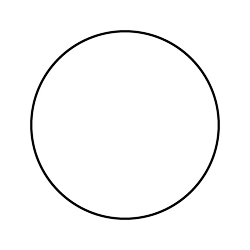
\includegraphics[width=\linewidth]{../data/virtual_0_1.png}
        \subcaption{$0_1$}
    \end{minipage}
    \begin{minipage}[b]{.14\linewidth}
        \centering
        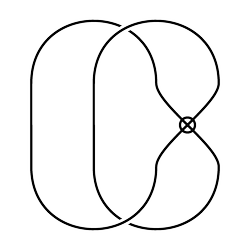
\includegraphics[width=\linewidth]{../data/virtual_2_1.png}
        \subcaption{$2_1$}
    \end{minipage}
    \begin{minipage}[b]{.14\linewidth}
        \centering
        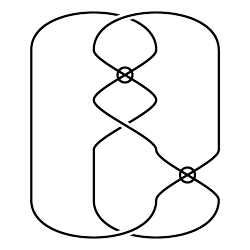
\includegraphics[width=\linewidth]{../data/virtual_3_1.png}
        \subcaption{$3_1$}
    \end{minipage}
    \begin{minipage}[b]{.14\linewidth}
        \centering
        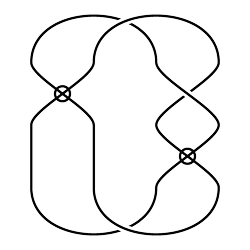
\includegraphics[width=\linewidth]{../data/virtual_3_7.png}
        \subcaption{$3_7$}
    \end{minipage}
    \begin{minipage}[b]{.14\linewidth}
        \centering
        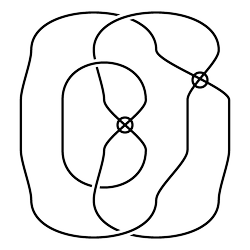
\includegraphics[width=\linewidth]{../data/virtual_4_1.png}
        \subcaption{$4_1$}
    \end{minipage}
    \begin{minipage}[b]{.14\linewidth}
        \centering
        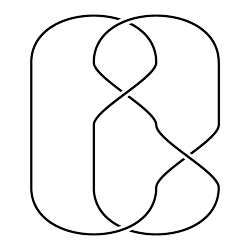
\includegraphics[width=\linewidth]{../data/virtual_4_108.png}
        \subcaption{$4_{108}$}
    \end{minipage}
    \caption{Garść węzłów osobliwych o małej liczbie skrzyżowań}
\end{figure}
\end{comment}

Podamy teraz definicję równoważności dla węzłów osobliwych, zupełnie analogicznie do definicji \ref{def:equivalent_knots_2} dla zwykłych węzłów.

\begin{definition}[płaski dysk]
    Niech $A$ będzie wierzchołkiem węzła osobliwego $K$, $B_A$ jego małym domkniętym otoczeniem, zaś $P_A$ płaszczyzną, która zawiera $B_A \cap K$, mały fragment węzła wokół wierzchołka.
    Dysk $P_A \cap B_A$ nazywamy płaskim dyskiem wokół wierzchołka $A$.
\end{definition}
% Murasugi

\begin{definition}
    Dwa osobliwe węzły $K, L$ są równoważne, co zapisujemy jako $K = L$, jeśli istnieje zachowujący orientację homeomorfizm $\varphi$ przestrzeni $\R^3$ w~siebie, który przenosi jeden węzeł na drugi: $\varphi(K) = L$ oraz indukuje bijekcję między rodzinami płaskich dysków $K$ i~$L$.
\end{definition}
% Murasugi

Ten drugi warunek gwarantuje nam, że skrzyżowania wokół podwójnych punktów nie ulegną zniszczeniu.
Istnieje podobne kryterium dla diagramów, odpowiednik twierdzenia Reidemeistera.

\begin{proposition}
\index{ruch!$\Omega$}%
\index{ruch!Reidemeistera}%
\index{twierdzenie!Reidemeistera}%
    Dwa osobliwe diagramy są równoważne dokładnie wtedy, kiedy można między nimi przejść przy użyciu ciągu izotopii otaczających, ruchów Reidemeistera, operacji $\Omega_4$ oraz $\Omega_5$.
\begin{comment}
    \begin{figure}[H]
    \centering
    \begin{minipage}[b]{.45\linewidth}
        \[
            \LargeVirtualReidemeisterThreeA \cong \LargeVirtualReidemeisterThreeB
        \]
        \subcaption{ruch $\Omega_{4a}$}
    \end{minipage}
    \begin{minipage}[b]{.45\linewidth}
        \[
            \LargeVirtualReidemeisterThreeC \cong \LargeVirtualReidemeisterThreeD
        \]
        \subcaption{ruch $\Omega_{4e}$}
    \end{minipage}
    \caption{Dwa osobliwe warianty III ruchu Reidemeistera}
    \end{figure}
    \begin{figure}[H]
        \[
            \LargeVirtualFlypeFiveA \cong \LargeVirtualFlypeFiveB
        \]
    \caption{Osobliwy wariant ruchu flype, $\Omega_5$}
    \end{figure}
\end{comment}
\end{proposition}

Uwaga: ufamy pracy Nelsona, Oyamaguchiego, Sazdanovic \cite{sazdanovic19} gdzie pokazano, że ten zestaw ruchów jest minimalny.
\index[persons]{Nelson, Sam}%
\index[persons]{Oyamaguchi, Natsumi}%
\index[persons]{Sazdanovic, Radmila}%
Natomist Murasugi podaje tylko jedną nową operację, wydaje nam się, że wszyscy nie mogą mieć racji.

Załóżmy teraz, że mamy jakiś niezmiennik węzłów $v$ o~wymiernych wartościach i~chcemy przedłużyć go do niezmiennika $\hat v$ węzłów osobliwych.
Najprościej zrobić to rekurencyjnie.
Niech $\hat v$ będzie już określony dla osobliwych węzłów o co najwyżej $n - 1$ wierzchołkach i~wybierzmy dowolny węzeł i diagram o~$n$ wierzchołkach.
Okazuje się, że jeżeli położymy

\begin{comment}
\begin{equation}
    \hat v\left( \MediumSingularCrossingArrows \right) =
    \hat v\left( \MediumPlusCrossingArrows \right) -
    \hat v\left( \MediumMinusCrossingArrows \right),
\end{equation}
\end{comment}
to dostaniemy dobrze określoną funkcję: jeżeli $L = K$ jest tym samym osobliwym węzłem z~innym diagramem, to $\hat v(L) = \hat v(K)$.
Funkcję $\hat v$ nazywamy niezmiennikiem osobliwym indukowanym przez niezmiennik węzłów $v_0$.

\begin{definition}[rząd niezmiennika]
\label{def:vassiliev_order}%
\index{niezmiennik!Wasiljewa!rząd ...}%
    Niech $v$ będzie niezmiennikiem osobliwym.
    Mówimy, że $v$ jest niezmiennikiem Wasiljewa rzędu co najwyżej $n$, jeśli dla dowolnego osobliwego węzła $K$ o $n + 1$ wierzchołkach zachodzi $v(K) = 0$.
    Jeśli dodatkowo $v$ nie jest rzędu co najwyżej $n - 1$, to mówimy, że jest rzędu dokładnie $n$.
\end{definition}

